\documentclass{article}\usepackage[]{graphicx}\usepackage[]{color}
%% maxwidth is the original width if it is less than linewidth
%% otherwise use linewidth (to make sure the graphics do not exceed the margin)
\makeatletter
\def\maxwidth{ %
  \ifdim\Gin@nat@width>\linewidth
    \linewidth
  \else
    \Gin@nat@width
  \fi
}
\makeatother

\definecolor{fgcolor}{rgb}{0.345, 0.345, 0.345}
\newcommand{\hlnum}[1]{\textcolor[rgb]{0.686,0.059,0.569}{#1}}%
\newcommand{\hlstr}[1]{\textcolor[rgb]{0.192,0.494,0.8}{#1}}%
\newcommand{\hlcom}[1]{\textcolor[rgb]{0.678,0.584,0.686}{\textit{#1}}}%
\newcommand{\hlopt}[1]{\textcolor[rgb]{0,0,0}{#1}}%
\newcommand{\hlstd}[1]{\textcolor[rgb]{0.345,0.345,0.345}{#1}}%
\newcommand{\hlkwa}[1]{\textcolor[rgb]{0.161,0.373,0.58}{\textbf{#1}}}%
\newcommand{\hlkwb}[1]{\textcolor[rgb]{0.69,0.353,0.396}{#1}}%
\newcommand{\hlkwc}[1]{\textcolor[rgb]{0.333,0.667,0.333}{#1}}%
\newcommand{\hlkwd}[1]{\textcolor[rgb]{0.737,0.353,0.396}{\textbf{#1}}}%

\usepackage{framed}
\makeatletter
\newenvironment{kframe}{%
 \def\at@end@of@kframe{}%
 \ifinner\ifhmode%
  \def\at@end@of@kframe{\end{minipage}}%
  \begin{minipage}{\columnwidth}%
 \fi\fi%
 \def\FrameCommand##1{\hskip\@totalleftmargin \hskip-\fboxsep
 \colorbox{shadecolor}{##1}\hskip-\fboxsep
     % There is no \\@totalrightmargin, so:
     \hskip-\linewidth \hskip-\@totalleftmargin \hskip\columnwidth}%
 \MakeFramed {\advance\hsize-\width
   \@totalleftmargin\z@ \linewidth\hsize
   \@setminipage}}%
 {\par\unskip\endMakeFramed%
 \at@end@of@kframe}
\makeatother

\definecolor{shadecolor}{rgb}{.97, .97, .97}
\definecolor{messagecolor}{rgb}{0, 0, 0}
\definecolor{warningcolor}{rgb}{1, 0, 1}
\definecolor{errorcolor}{rgb}{1, 0, 0}
\newenvironment{knitrout}{}{} % an empty environment to be redefined in TeX

\usepackage{alltt}
\usepackage{enumerate}
\usepackage{amsmath}
\IfFileExists{upquote.sty}{\usepackage{upquote}}{}
\begin{document}

\title{\huge \textbf{Stat 207 HW8} \\}
\author{\large Cheng Luo 912466499 \\ \large Fan Wu 912538518}
\maketitle

\newpage
\mbox{}
\newpage


\section{14.28}

\begin{enumerate}[(a)]

\item

\begin{knitrout}
\definecolor{shadecolor}{rgb}{0.969, 0.969, 0.969}\color{fgcolor}\begin{kframe}
\begin{alltt}
  \hlstd{dat} \hlkwb{=} \hlkwd{read.table}\hlstd{(}\hlstr{"CH14PR14.txt"}\hlstd{)}
  \hlkwd{names}\hlstd{(dat)} \hlkwb{=} \hlkwd{c}\hlstd{(}\hlstr{"Y"}\hlstd{,} \hlstr{"X1"}\hlstd{,} \hlstr{"X2"}\hlstd{,} \hlstr{"X3"}\hlstd{)}
  \hlstd{logit} \hlkwb{=} \hlkwd{glm}\hlstd{(Y} \hlopt{~} \hlstd{X1} \hlopt{+} \hlstd{X2 ,} \hlkwc{data} \hlstd{= dat,} \hlkwc{family} \hlstd{=} \hlstr{"binomial"}\hlstd{)}
  \hlstd{logitv} \hlkwb{=} \hlstd{logit}\hlopt{$}\hlstd{fitted.values}
  \hlstd{dat} \hlkwb{=} \hlstd{dat[}\hlkwd{order}\hlstd{(logitv), ]}
  \hlstd{a} \hlkwb{=} \hlkwd{rep}\hlstd{(}\hlnum{1}\hlopt{:}\hlnum{8}\hlstd{,} \hlkwc{each} \hlstd{=} \hlnum{20}\hlstd{)}
  \hlstd{a} \hlkwb{=} \hlstd{a[}\hlopt{-}\hlnum{1}\hlstd{]}
  \hlstd{b} \hlkwb{=} \hlkwd{split}\hlstd{(dat, a)}
  \hlstd{Oj1} \hlkwb{=} \hlkwd{sapply}\hlstd{(b,} \hlkwa{function}\hlstd{(}\hlkwc{x}\hlstd{)\{}\hlkwd{sum}\hlstd{(x[[}\hlnum{1}\hlstd{]])\})}
  \hlstd{Ej1} \hlkwb{=} \hlkwd{sapply}\hlstd{(}\hlkwd{split}\hlstd{(}\hlkwd{sort}\hlstd{(logitv), a), sum)}
  \hlstd{Oj0} \hlkwb{=} \hlkwd{sapply}\hlstd{(b,} \hlkwa{function}\hlstd{(}\hlkwc{x}\hlstd{)\{}\hlkwd{length}\hlstd{(x[[}\hlnum{1}\hlstd{]])}\hlopt{-}\hlkwd{sum}\hlstd{(x[[}\hlnum{1}\hlstd{]])\})}
  \hlstd{Ej0} \hlkwb{=} \hlkwd{sapply}\hlstd{(b,} \hlkwa{function}\hlstd{(}\hlkwc{x}\hlstd{)\{}\hlkwd{length}\hlstd{(x[[}\hlnum{1}\hlstd{]])\})}\hlopt{-}\hlstd{Ej1}
  \hlkwd{rbind}\hlstd{(Oj1, Ej1, Oj0, Ej0)}
\end{alltt}
\begin{verbatim}
##             1          2          3         4         5        6         7
## Oj1  0.000000  1.0000000  0.0000000  2.000000  1.000000  8.00000  2.000000
## Ej1  0.187472  0.5159059  0.9878718  1.512501  2.412695  3.44151  4.680125
## Oj0 19.000000 19.0000000 20.0000000 18.000000 19.000000 12.00000 18.000000
## Ej0 18.812528 19.4840941 19.0121282 18.487499 17.587305 16.55849 15.319875
##             8
## Oj1 10.000000
## Ej1 10.261919
## Oj0 10.000000
## Ej0  9.738081
\end{verbatim}
\begin{alltt}
  \hlstd{x} \hlkwb{=} \hlkwd{sapply}\hlstd{(}\hlkwd{split}\hlstd{(}\hlkwd{sort}\hlstd{(logitv), a), median)}
  \hlstd{y} \hlkwb{=} \hlstd{Ej1}\hlopt{/}\hlkwd{sapply}\hlstd{(b,} \hlkwa{function}\hlstd{(}\hlkwc{x}\hlstd{)\{}\hlkwd{length}\hlstd{(x[[}\hlnum{1}\hlstd{]])\})}
  \hlkwd{plot}\hlstd{(x, y)}
\end{alltt}
\end{kframe}
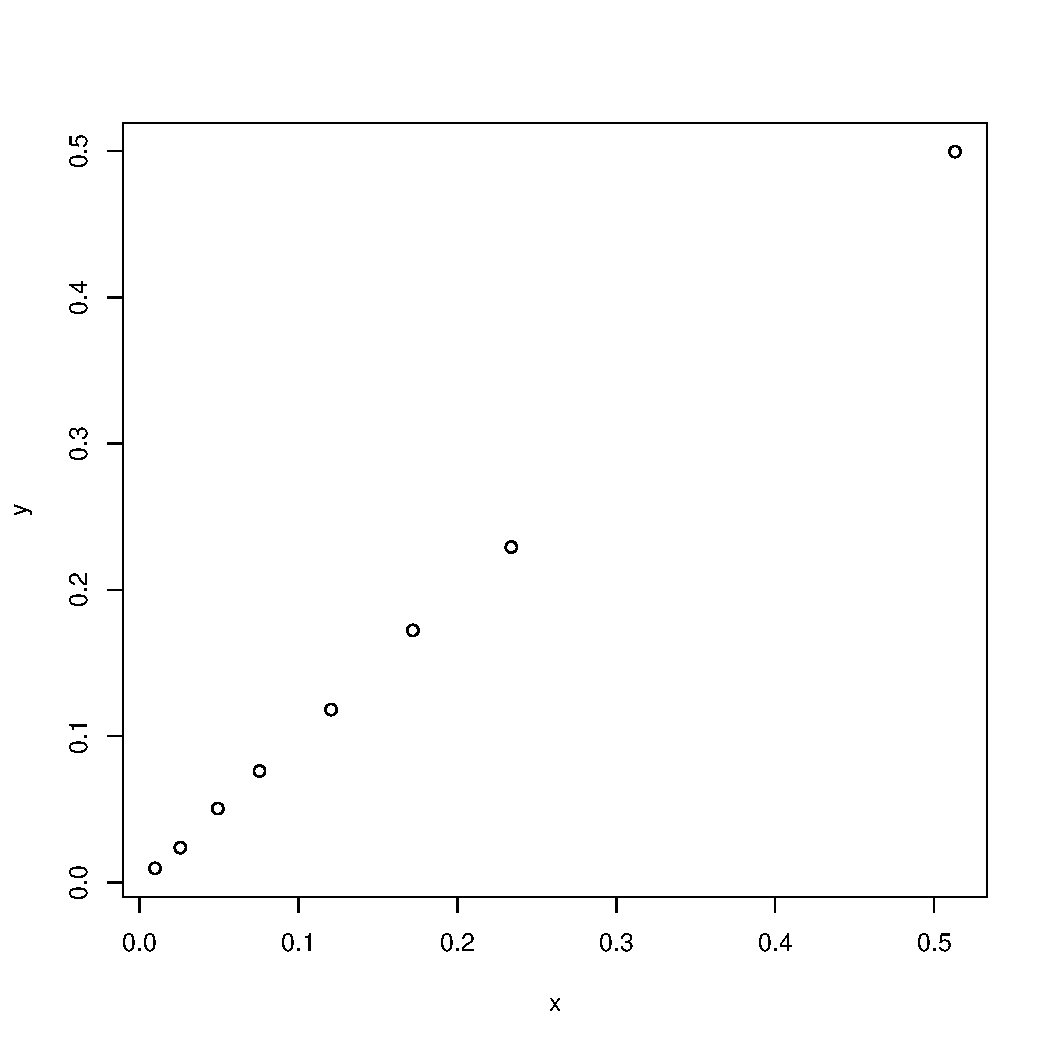
\includegraphics[width=\maxwidth]{figure/unnamed-chunk-1-1} 

\end{knitrout}

\qquad The plot seems to be linear, it's consistent with a response function of monotonic sigmoidal shape.

\item

\begin{knitrout}
\definecolor{shadecolor}{rgb}{0.969, 0.969, 0.969}\color{fgcolor}\begin{kframe}
\begin{alltt}
  \hlstd{X.squ} \hlkwb{=} \hlkwd{sum}\hlstd{((}\hlkwd{rbind}\hlstd{(Oj1, Oj0)}\hlopt{-}\hlkwd{rbind}\hlstd{(Ej1, Ej0))}\hlopt{^}\hlnum{2}\hlopt{/}\hlkwd{rbind}\hlstd{(Ej1, Ej0));X.squ}
\end{alltt}
\begin{verbatim}
## [1] 12.11578
\end{verbatim}
\end{kframe}
\end{knitrout}

\begin{center}
$H_0$:$E(Y)=[1+exp(-\beta_0-\beta_1 X1-\beta_2 X2)]^{-1}$

VS. $H_1$:$E(Y)  \ne [1+exp(-\beta_0-\beta_1 X1-\beta_2 X2)]^{-1}$

$X^2=\sum_j \sum_k \frac{(O_{jk}-E_{jk})^2}{E_{jk}} = 12.11578$

we can reject $H_0$ if $X^2 > \chi^2(0.95, 8-3)=11.0705$,otherwise reject$H_1$

so that reject $H_0$ because $X^2 >11.0705$, Pvalue is 0.03323531.
\end{center}

\item

\begin{knitrout}
\definecolor{shadecolor}{rgb}{0.969, 0.969, 0.969}\color{fgcolor}\begin{kframe}
\begin{alltt}
  \hlstd{p} \hlkwb{=} \hlkwd{summary}\hlstd{(logit)}
  \hlstd{dr} \hlkwb{=} \hlstd{p}\hlopt{$}\hlstd{deviance.resid;dr}
\end{alltt}
\begin{verbatim}
##           1           2           3           4           5           6 
## -0.54602312 -0.51373259  1.15260237 -0.17517944 -0.18924467 -0.69185916 
##           7           8           9          10          11          12 
## -0.18367445 -0.73777334 -0.47288089 -0.35855218 -0.62785882 -0.33244658 
##          13          14          15          16          17          18 
## -0.49058859 -0.23345211 -0.11467682 -0.59485941 -0.85058862 -0.16214474 
##          19          20          21          22          23          24 
## -0.22270681 -0.13939895 -0.34822874 -0.28168748 -0.24470112 -0.09084127 
##          25          26          27          28          29          30 
## -0.50595282 -0.10798927 -0.69416101 -0.26781191 -0.83451488 -0.68109529 
##          31          32          33          34          35          36 
## -0.32519247 -0.45851859 -0.92893094 -0.53211206 -0.33897782 -0.16073331 
##          37          38          39          40          41          42 
##  0.74365705  1.38971984 -0.61999873 -0.41310085  1.89079347 -0.35679774 
##          43          44          45          46          47          48 
##  1.71627562 -0.33244658 -0.72647043 -0.32961191  2.84304938 -0.69729005 
##          49          50          51          52          53          54 
## -0.10990097 -0.18854516 -0.33530428 -0.21617318 -0.72171075 -0.59079687 
##          55          56          57          58          59          60 
##  2.23462510 -0.24806553 -0.42012390 -0.28029236 -1.30166964  2.00689554 
##          61          62          63          64          65          66 
##  1.10849910 -0.15933400 -0.68109529 -0.32124458 -0.10387671 -1.01249619 
##          67          68          69          70          71          72 
## -0.12087236 -0.36424502 -0.62497861  1.86302691 -0.23960963 -0.48311783 
##          73          74          75          76          77          78 
## -0.38006335  1.82187884 -1.44789883 -0.84697959 -0.83715068 -0.35248880 
##          79          80          81          82          83          84 
## -0.58403320 -0.45631940 -0.35855218  1.94481807 -0.72970910 -0.53462959 
##          85          86          87          88          89          90 
## -0.36293048 -1.15124676 -0.62286031 -0.65995923  2.34647993 -0.81345988 
##          91          92          93          94          95          96 
##  1.12311780 -0.17737218  1.27437628 -0.55762351 -0.49703364 -0.30029670 
##          97          98          99         100         101         102 
## -1.06493877 -0.71059309  0.95982139 -0.33201751 -0.67802259  1.90510957 
##         103         104         105         106         107         108 
## -0.45631940 -0.42162878 -0.12900059 -0.17648324 -0.19257415 -0.14876060 
##         109         110         111         112         113         114 
##  1.82969794 -0.32283373 -0.53091804 -0.13409993 -0.61013597 -0.72086770 
##         115         116         117         118         119         120 
## -0.50887859 -0.61087534 -0.16356841 -0.16073331 -0.12675915 -0.49293406 
##         121         122         123         124         125         126 
## -0.14931436 -0.21351074  1.84295971 -0.40421564  1.40875849 -0.30814469 
##         127         128         129         130         131         132 
## -0.40618549 -0.49528940 -0.51130056 -0.73777334 -0.28412789 -0.58877426 
##         133         134         135         136         137         138 
## -0.49703364 -1.22831729 -0.31850052  1.89079347 -0.29409388 -0.69416101 
##         139         140         141         142         143         144 
## -0.20982689 -0.48482421 -0.61925036 -0.28658859 -0.39176366 -0.48311783 
##         145         146         147         148         149         150 
## -1.11866815 -0.31307905 -0.35422338 -0.28065744 -0.72970910 -0.20982689 
##         151         152         153         154         155         156 
## -0.41110024 -0.42725579 -0.28554134 -0.38936035 -0.29263987 -0.25647527 
##         157         158         159 
##  0.42476809  0.86785144  1.67453806
\end{verbatim}
\begin{alltt}
  \hlstd{pi} \hlkwb{=} \hlkwd{exp}\hlstd{(logitv)}\hlopt{/}\hlstd{(}\hlnum{1}\hlopt{+}\hlkwd{exp}\hlstd{(logitv))}
  \hlkwd{plot}\hlstd{(}\hlkwd{lowess}\hlstd{(dr} \hlopt{~} \hlstd{pi))}
\end{alltt}
\end{kframe}
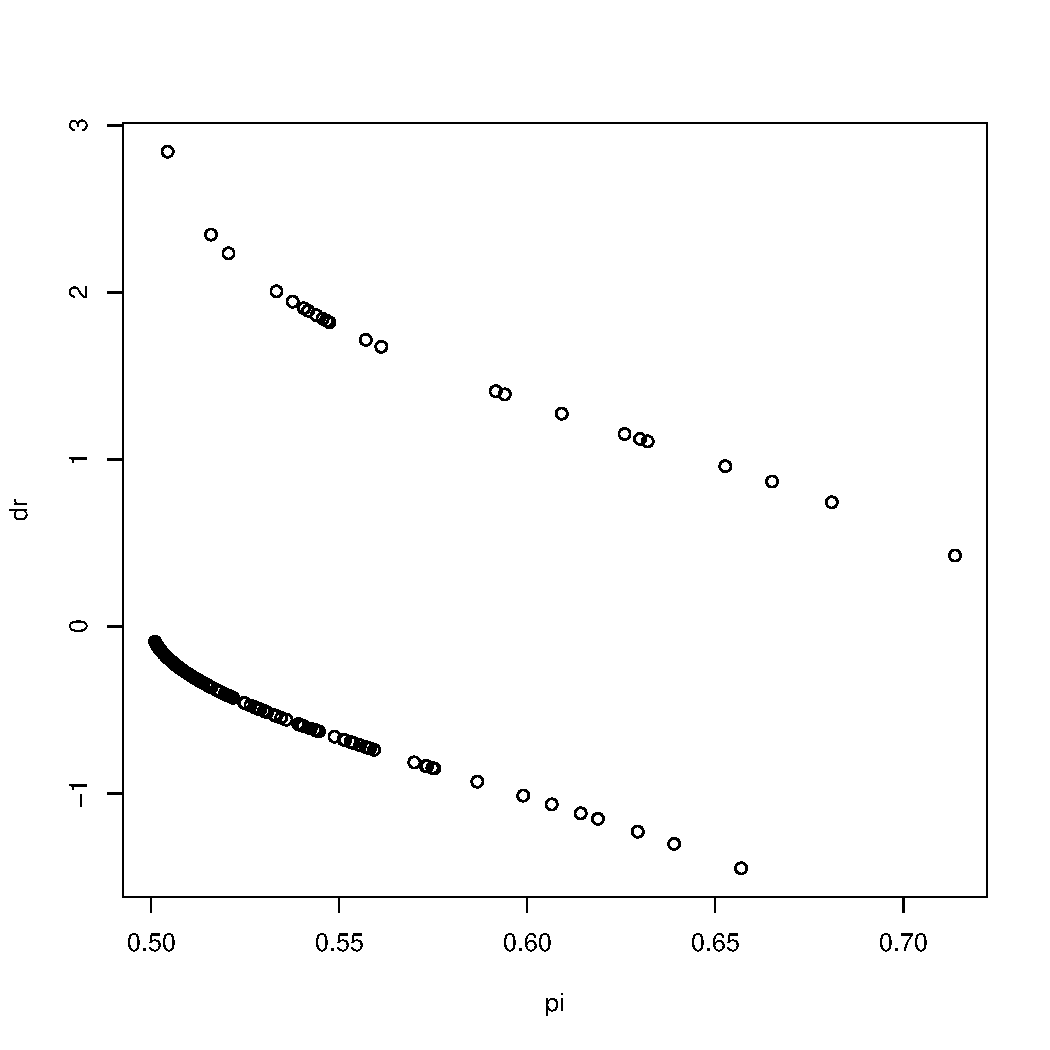
\includegraphics[width=\maxwidth]{figure/unnamed-chunk-3-1} 

\end{knitrout}

\qquad

\end{enumerate}

\section{14.39}

\begin{enumerate}[(a)]

\item

\begin{knitrout}
\definecolor{shadecolor}{rgb}{0.969, 0.969, 0.969}\color{fgcolor}\begin{kframe}
\begin{alltt}
  \hlstd{dat} \hlkwb{=} \hlkwd{read.table}\hlstd{(}\hlstr{"CH14PR39.txt"}\hlstd{)}
  \hlkwd{names}\hlstd{(dat)} \hlkwb{=} \hlkwd{c}\hlstd{(}\hlstr{"Y"}\hlstd{,} \hlstr{"X1"}\hlstd{,} \hlstr{"X2"}\hlstd{,} \hlstr{"X3"}\hlstd{,} \hlstr{"X4"}\hlstd{)}
  \hlstd{poi} \hlkwb{=} \hlkwd{glm}\hlstd{(Y} \hlopt{~} \hlstd{. ,} \hlkwc{data} \hlstd{= dat,} \hlkwc{family} \hlstd{=} \hlstr{"poisson"}\hlstd{)}
  \hlkwd{summary}\hlstd{(poi)}
\end{alltt}
\begin{verbatim}
## 
## Call:
## glm(formula = Y ~ ., family = "poisson", data = dat)
## 
## Deviance Residuals: 
##     Min       1Q   Median       3Q      Max  
## -2.1854  -0.7819  -0.2564   0.5449   2.3626  
## 
## Coefficients:
##              Estimate Std. Error z value Pr(>|z|)    
## (Intercept)  0.489467   0.336869   1.453  0.14623    
## X1          -1.069403   0.133154  -8.031 9.64e-16 ***
## X2          -0.046606   0.119970  -0.388  0.69766    
## X3           0.009470   0.002953   3.207  0.00134 ** 
## X4           0.008566   0.004312   1.986  0.04698 *  
## ---
## Signif. codes:  0 '***' 0.001 '**' 0.01 '*' 0.05 '.' 0.1 ' ' 1
## 
## (Dispersion parameter for poisson family taken to be 1)
## 
##     Null deviance: 199.19  on 99  degrees of freedom
## Residual deviance: 108.79  on 95  degrees of freedom
## AIC: 377.29
## 
## Number of Fisher Scoring iterations: 5
\end{verbatim}
\end{kframe}
\end{knitrout}

\begin{displaymath}
\begin{split}
  b_0 = 0.489467 &\qquad s(b_0)=0.336869 \\
  b_1 = -1.069403 &\qquad  s(b_1)=0.133154 \\
  b_2 = -0.046606 &\qquad  s(b_2)=0.119970 \\
  b_3 = 0.009470 &\qquad  s(b_3)=0.002953 \\
  b_4 = 0.008566 &\qquad  s(b_4)=0.004312 \\
  \mu = exp(0.489467165 -1.069402551 X1 & -0.046606063 X2 +  0.009469987X3 +  0.008565829 X4)
\end{split}
\end{displaymath}

\item

\begin{knitrout}
\definecolor{shadecolor}{rgb}{0.969, 0.969, 0.969}\color{fgcolor}\begin{kframe}
\begin{alltt}
  \hlstd{p} \hlkwb{=} \hlkwd{summary}\hlstd{(poi)}
  \hlstd{dr} \hlkwb{=} \hlstd{p}\hlopt{$}\hlstd{deviance.resid;dr}
\end{alltt}
\begin{verbatim}
##            1            2            3            4            5 
## -0.481563003 -0.632820229  0.485684782 -1.819828480  0.238302497 
##            6            7            8            9           10 
## -0.427206484 -1.574566470 -1.694831446 -0.190494237  0.372414202 
##           11           12           13           14           15 
##  0.290568448  0.917894609  0.618945304  0.710218879 -0.169117683 
##           16           17           18           19           20 
##  0.774212615  1.313966589  0.976533023 -0.284161510  0.281078819 
##           21           22           23           24           25 
##  0.671826155 -0.309823439 -0.585274974 -1.659501048 -1.653549229 
##           26           27           28           29           30 
##  0.545695411 -2.089197070 -1.825162331  0.283158353  1.066089357 
##           31           32           33           34           35 
##  0.338495236 -0.414912576 -0.276062096  2.097482057 -0.373770021 
##           36           37           38           39           40 
## -2.185378873  2.217373787 -0.269196968 -1.468917177 -0.490568471 
##           41           42           43           44           45 
## -0.243689445  2.287659410 -0.435460637 -0.171363655 -1.596370920 
##           46           47           48           49           50 
##  0.178588604 -1.840819930  1.313615961 -0.233624875 -1.576829772 
##           51           52           53           54           55 
## -0.652282150  2.177759158 -0.862317963 -1.223172388 -0.161565009 
##           56           57           58           59           60 
## -0.438457085 -0.817656201  0.002451800 -0.690070466 -0.932653968 
##           61           62           63           64           65 
## -0.532725622  0.400431092  1.326821516  0.569505372  0.589162479 
##           66           67           68           69           70 
##  0.222202292  1.991163395  0.134986579  1.163783804  0.890153115 
##           71           72           73           74           75 
## -0.398888037 -0.335860573 -0.843868576  1.065308951 -0.068529260 
##           76           77           78           79           80 
## -1.210403791  0.928316209 -0.803424449 -0.050707876 -0.817762385 
##           81           82           83           84           85 
##  0.544674549 -1.761754891 -0.562223893 -0.541853422  0.147418906 
##           86           87           88           89           90 
## -0.009840529 -0.337422359 -0.774688780 -1.383658148 -0.654757856 
##           91           92           93           94           95 
## -1.475851025 -0.722343228  2.362545161  1.391144309  1.262066676 
##           96           97           98           99          100 
##  0.117099736 -0.827717570 -0.345172951  0.048822205 -0.988857456
\end{verbatim}
\begin{alltt}
  \hlkwd{plot}\hlstd{(}\hlkwd{sort}\hlstd{(dr))}
\end{alltt}
\end{kframe}
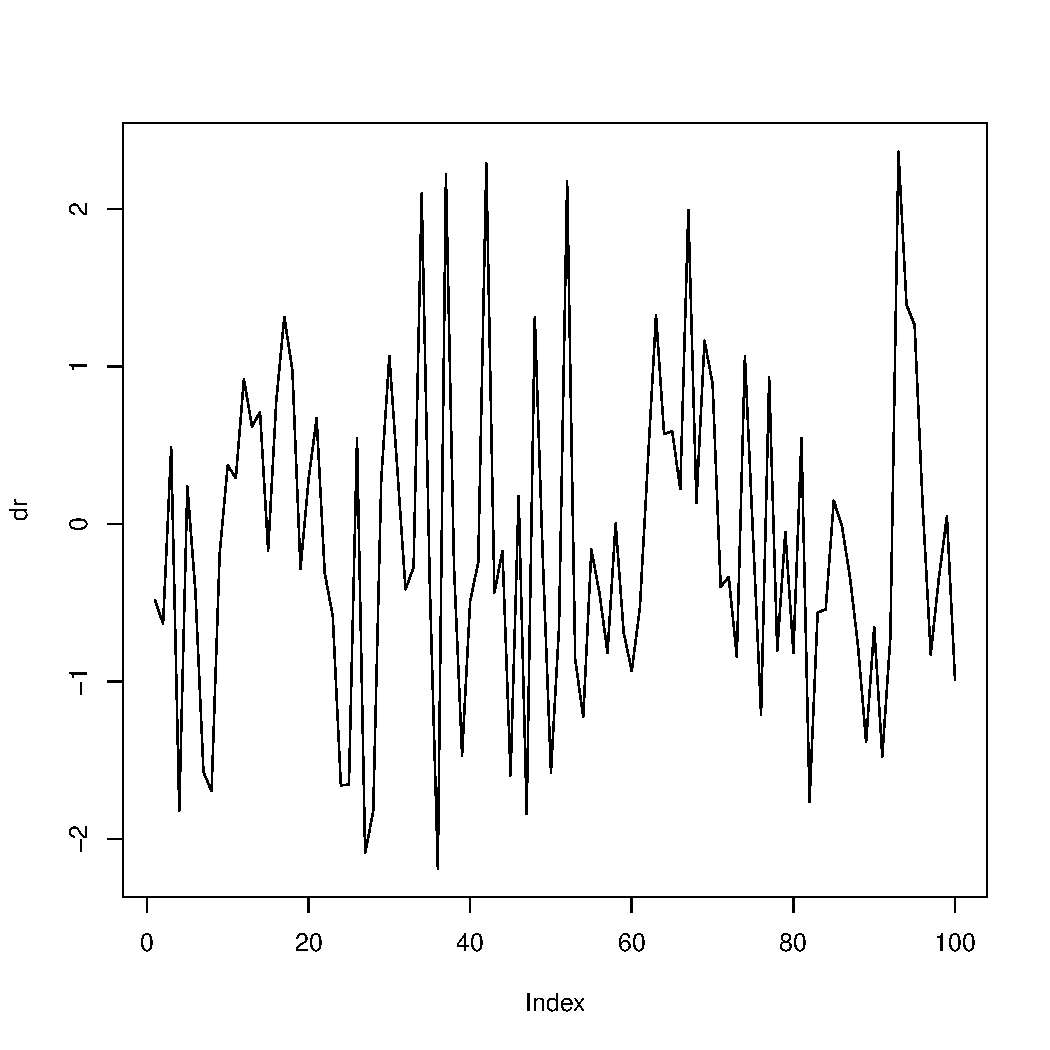
\includegraphics[width=\maxwidth]{figure/unnamed-chunk-5-1} 

\end{knitrout}

\qquad The points whose devaiance residual near 100 seem to be outlyers.

\item

\begin{knitrout}
\definecolor{shadecolor}{rgb}{0.969, 0.969, 0.969}\color{fgcolor}\begin{kframe}
\begin{alltt}
  \hlkwd{logLik}\hlstd{(poi)}
\end{alltt}
\begin{verbatim}
## 'log Lik.' -183.6439 (df=5)
\end{verbatim}
\begin{alltt}
  \hlstd{poiR} \hlkwb{=} \hlkwd{glm}\hlstd{(Y} \hlopt{~} \hlstd{.}\hlopt{-}\hlstd{X2 ,} \hlkwc{data} \hlstd{= dat,} \hlkwc{family} \hlstd{=} \hlstr{"poisson"}\hlstd{)}
  \hlkwd{logLik}\hlstd{(poiR)}
\end{alltt}
\begin{verbatim}
## 'log Lik.' -183.7194 (df=4)
\end{verbatim}
\begin{alltt}
  \hlkwd{qchisq}\hlstd{(}\hlnum{1}\hlopt{-}\hlnum{0.05}\hlstd{,} \hlnum{5}\hlopt{-}\hlnum{4}\hlstd{)}
\end{alltt}
\begin{verbatim}
## [1] 3.841459
\end{verbatim}
\begin{alltt}
  \hlkwd{pchisq}\hlstd{(}\hlnum{0.151}\hlstd{,} \hlnum{1}\hlstd{,} \hlkwc{lower.tail} \hlstd{=} \hlnum{FALSE}\hlstd{)}
\end{alltt}
\begin{verbatim}
## [1] 0.6975815
\end{verbatim}
\end{kframe}
\end{knitrout}

\begin{center}
$H_0$:$\beta_2=0$

VS. $H_1$:$\beta_2 \ne 0$

The full model: $\mu = exp(\beta_0 + \beta_1 X1 + \beta_2 X2 + \beta_3 X3 + \beta_4 X4) $

ln(L(F))= -183.6439

The reduced model: $\mu = exp(\beta_0 + \beta_1 X1 + \beta_3 X3 + \beta_4 X4) $

ln(L(R))= -183.7194

$G^2$ = -2(ln(L(R)-ln(L(F)))) = 0.151

we can reject $H_0$ if $G^2 > \chi^2(1-0.05, 5-4)=3.8415$,otherwise reject$H_1$

so that reject $H_1$ because $G^2 < 3.8415$,

therefore, X2 can be dropped from the regression model, and the P-value is 0.6975815.And the result is the same as the result we get in (b).
\end{center}

\item

\begin{knitrout}
\definecolor{shadecolor}{rgb}{0.969, 0.969, 0.969}\color{fgcolor}\begin{kframe}
\begin{alltt}
  \hlkwd{summary}\hlstd{(poiR)}
\end{alltt}
\begin{verbatim}
## 
## Call:
## glm(formula = Y ~ . - X2, family = "poisson", data = dat)
## 
## Deviance Residuals: 
##     Min       1Q   Median       3Q      Max  
## -2.2152  -0.7512  -0.2594   0.5830   2.2893  
## 
## Coefficients:
##              Estimate Std. Error z value Pr(>|z|)    
## (Intercept)  0.443890   0.317289   1.399  0.16181    
## X1          -1.077770   0.131415  -8.201 2.38e-16 ***
## X3           0.009471   0.002957   3.203  0.00136 ** 
## X4           0.008979   0.004190   2.143  0.03209 *  
## ---
## Signif. codes:  0 '***' 0.001 '**' 0.01 '*' 0.05 '.' 0.1 ' ' 1
## 
## (Dispersion parameter for poisson family taken to be 1)
## 
##     Null deviance: 199.19  on 99  degrees of freedom
## Residual deviance: 108.94  on 96  degrees of freedom
## AIC: 375.44
## 
## Number of Fisher Scoring iterations: 5
\end{verbatim}
\begin{alltt}
  \hlstd{b1} \hlkwb{=} \hlopt{-}\hlnum{1.077770}
  \hlstd{s1} \hlkwb{=} \hlnum{0.131415}
  \hlstd{z} \hlkwb{=} \hlkwd{qnorm}\hlstd{(}\hlnum{1}\hlopt{-}\hlnum{0.05}\hlopt{/}\hlnum{2}\hlstd{)}
  \hlkwd{c}\hlstd{(b1}\hlopt{-}\hlstd{s1}\hlopt{*}\hlstd{z, b1}\hlopt{+}\hlstd{s1}\hlopt{*}\hlstd{z)}
\end{alltt}
\begin{verbatim}
## [1] -1.3353387 -0.8202013
\end{verbatim}
\end{kframe}
\end{knitrout}

\qquad From summary(poiR), we get $s(b_1) = 0.131415, b_1 = -1.077770$, based on $b_k \pm z(1-\alpha/2)s{b_k}$, we conclude that we are 95 \% confident that $\beta_1$ is between -1.3353387 and -0.8202013. Because the confidence interval is smaller than 0, aerobic exercise reduce the frequency of falls when controlling for balance and strength.

\end{enumerate}

\section{14.44}

\section{14.45}

\section{14.46}

\begin{displaymath}
\begin{split}
  E(Y) &= [1 + exp(-\beta_0-\beta_1 X_1 - \beta_2 X_2 - \beta_3 X_1 X_2)]^{-1} \\
  \pi^{'}(X_1)  &= \beta_0 + \beta_1 X_1 + \beta_2 X_2 + \beta_3 X_1 X_2 \\
  \pi^{'}(X_1 + 1)  &= \beta_0 + \beta_1 (X_1 + 1) + \beta_2 X_2 + \beta_3 (X_1 + 1) X_2 \\ 
  \pi^{'}(X_1 + 1) - \pi^{'}(X_1) &= ln(odds ratio) = \beta_1 X_1 + \beta_3 X_1 X_2\\
  \text{ Hence the odds ratio for X1 is } & exp(\beta_1 X_1 + \beta_3 X_1 X_2) \text{therefore, they are different.} \\
\end{split}
\end{displaymath}

\section{14.47}

\end{document}
